
\documentclass[../main.tex]{subfiles}

\begin{document}


Pattern matching is a fundamental string processing problem. Pattern matching algorithms are also called string searching algorithms, and it is defined a class of string algorithms that try to find a place where one or several strings (also called patterns) are found within a larger string or text. Based on if some mismathces are allowed or not, we have \textbf{Exact or Approximate} Pattern Matching. In this section, we start from exact single-pattern matching algorithms where we only need to find one pattern in a given string or text. 
Based on how on how many patterns we might have, we have \textbf{one-time or multiple-times} string pattern matching problems. For multiple-times matching, preprocessing the text using suffix array/trie/tree can improve the total efficiency.  This chapter is organized as:
\begin{enumerate}
    \item Exact Pattern Matching: includes one-pattern and multiple patterns. 
    \item Approximate Pattern Matching:
\end{enumerate}


\section{Exact Single-Pattern Matching}

\paragraph{Exact Single-pattern Matching Problem}  Given two strings or two arrays, one is pattern \textbf{P} which has size $m$, and the other is the target string or text \textbf{T} which has size $n$, the exact single-pattern matching problem is defined as finding the first one or all occurrences of pattern P in the T as substring, and return the starting indexes of all the occurrences. 

\begin{figure}[h]
    \centering
    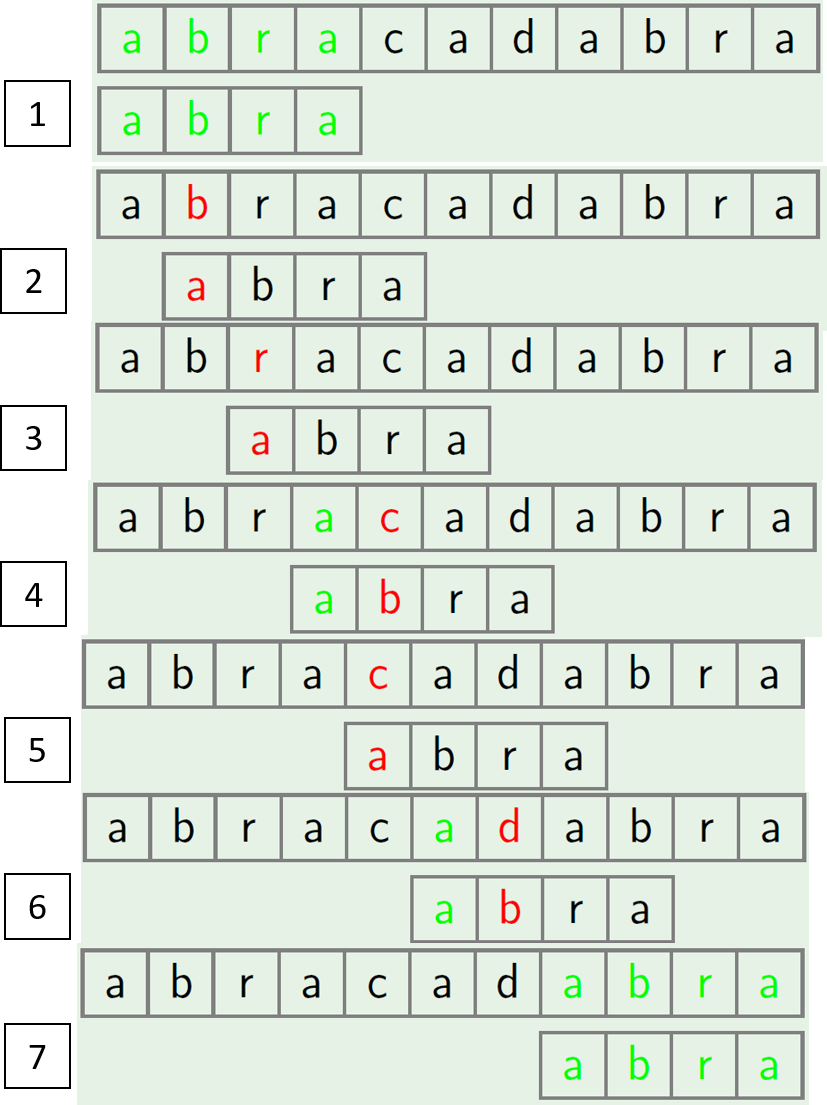
\includegraphics[width = 0.7\columnwidth]{fig/brute_force_matching.png}
    \caption{The process of the brute force exact pattern matching}
    \label{fig:brute_force_string_matching}
\end{figure}

\paragraph{Brute Force Solution} The naive searching is straightforward, we slide the pattern P like sliding window algorithm through the text T one by one item. At each position $i$, we compare P with T[i:i+m]. In this process, we need to do $n-m$ times of comparison, and each comparison takes maximum of $m$ times of computation. This brute force solution gives $O(mn)$ time complexity.
\begin{lstlisting}[language=Python]
def bruteForcePatternMatching(p, s):
    if len(p) > len(s):
        return [-1]
    m, n = len(p), len(s)
    ans = []
    for i in range(n-m+1):
        if s[i:i+m] == p:
            ans.append(i)
    return ans
    
p = "AABA"
s = "AABAACAADAABAABA"
print(bruteForcePatternMatching(p,s))
# output
# [0, 9, 12]
\end{lstlisting}
We write it in another way that use less built-in python function:
\begin{lstlisting}[language=Python]
def bruteForcePatternMatchingAll(p, s):
    if not s or not p:
        return []
    m, n = len(p), len(s)
    i, j = 0, 0
    ans = []
    while i < n:
        # do the pattern matching  
        if s[i] == p[j]:
            i += 1
            j += 1
            if j == m: #collect position
                ans.append(i - j)
                i = i-j+1
                j = 0
        else:
            i = i -j + 1
            j = 0
    return ans
\end{lstlisting}

For LeetCode Problems, most times, brute force solution will not be accepted and receive LTE. In real applications, such as human genome matching, the text can have approximate size of $3*10^9$ and the pattern can be very long to, such as $10^8$. Therefore, other faster algorithms are needed to improve the efficiency. 

The other algorithms requires us preprocess either/both the pattern and text. In this book, we mainly discuss three algorithms:
\begin{enumerate}
    \item Knuth Morris Pratt (KMP) Algorithm (Section~\ref{pattern_matching_subsec_kmp}). KMP is  a linear algorithm, and it should mostly be enough to solve interview related string matching, and also once we understand the algorithm, the implementation is quite trivial, which makes it a very good algorithm during interviews. It has $O(m+n)$ and $O(m)$ in the case of the time and space complexity.
    \item Suffix Trie/Tree/Array Matching (Section~\ref{pattern_matching_subsec_suffix_array}).
\end{enumerate}
%%%%%%%%%%%%%%%%%%%%%%%%%%%%%%%%%%%%%%%%%%%%%%%%%%%%%%%%%%%%%%%%%%%%%%%%%%%
%%%%% Knuth Morris Pratt
%%%%%%%%%%%%%%%%%%%%%%%%%%%%%%%%%%%%%%%%%%%%%%%%%%%%%%%%%%%%%%%%%%%%%%%%%%%
\subsection{Prefix Function and Knuth Morris Pratt (KMP)}
\label{pattern_matching_subsec_kmp}
In the above brute force solution, we compare our pattern with each item as starting window in the text. Each matching result is independent of each other, which is a lot of information lose to improve the efficiency. 

\paragraph{Skipping Positions} See Fig.~\ref{fig:brute_force_string_matching}, we know a matching at step 1. Is it necessary for us to do step 2 and step 3? The pattern itself tells us it is impossible to get a match at step 2 and step 3 because 'b' will dismatch 'a' and 'r' will dismatch 'a' too. However, at the original step 4, by analyzing the pattern itself we know 'a' will match 'a', and any step further, we have not enough information to cover, therefore, step 4 is necessary to compare 'c' with 'b' in the pattern. In this example, step 4, 5, 6, 7 are all needed but step 4, 5, 6 will only end up do one or two comparison each step. 

\begin{figure}[h]
    \centering
    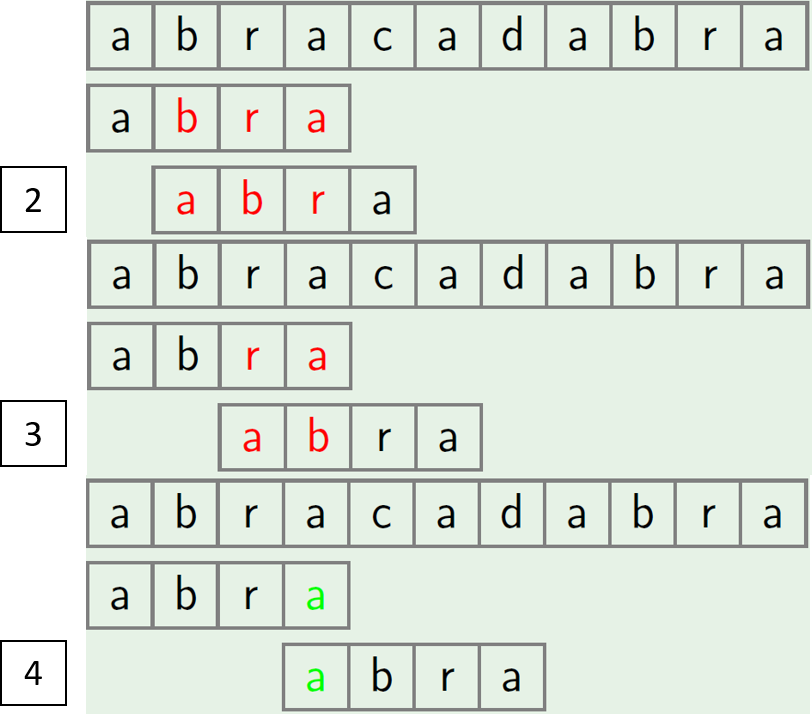
\includegraphics[width = 0.7\columnwidth]{fig/skipping_rule_kmp.png}
    \caption{The Skipping Rule}
    \label{fig:skipping_rule_kmp}
\end{figure}

 The reason why step 2 and 3 can be skipped can be shown from Fig.~\ref{fig:skipping_rule_kmp}. If we analyze our pattern at first, we will know at step 2 and step 3, ``bra'' not equals to ``abr'' and ``ra'' not equals to ``ab''. While at step 4, we do have ``a'' equals to ``a''. If we observe further of the relations of these pairs, we will know they are suffix and prefix of the same length of the pattern. Inspired by this, we define \textbf{border} of string S as a prefix of S which is equals to a suffix of the same length of S, but not equals to the whole S. For example:
 \begin{lstlisting}[numbers=none]
 ''a'' is a border of 'arba'
 'ab' is a border of 'abcdab'
 'ab' is not a border of 'ab'
 \end{lstlisting}
 
\begin{figure}[h]
    \centering
    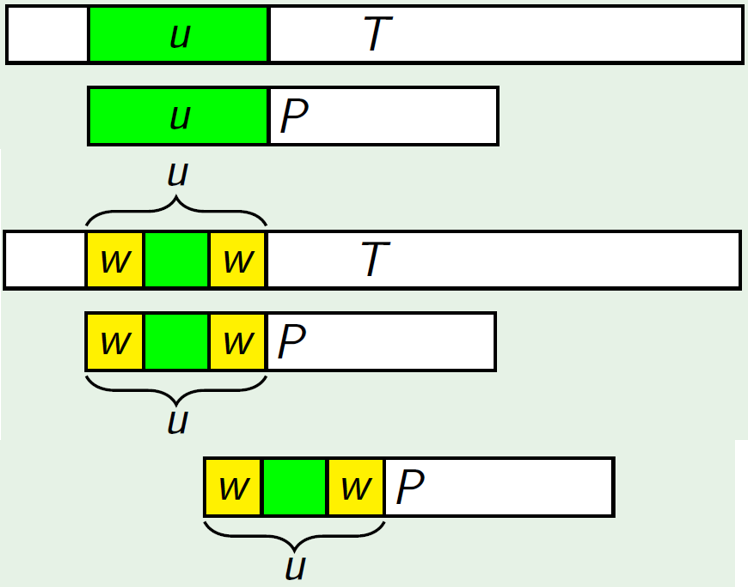
\includegraphics[width = 0.7\columnwidth]{fig/shifing_pattern.png}
    \caption{The Sliding Rule}
    \label{fig:sliding_rule_kmp}
\end{figure}

%\url{https://cp-algorithms.com/string/prefix-function.html}
\paragraph{Prefix Function} A Prefix function for a string P generates an array $l$ (lps is short for failure loopkp table) of the same length of string, where $lps[i]$ is the length of the longest border of for prefix substring P[0...i]. Mathematically the definition of prefix function can be written as follows:
\begin{equation}
    l[i] = \max_{k=0,...,i}\{k: P[0...k-1] = P[i-(k-1)...i\}
\end{equation}
The naive implementation of prefix-function takes $O(n^3)$:
\begin{lstlisting}[language=Python]
def naiveLps(p:str):
  dp = [0] * len(p)
  for i in range(1, len(p)):
    for l in range(i, 0, -1): # from maxmim length to length 1
      prefix = p[0: l]
      suffix = p[i - l+1: i+1]
      #print(prefix, suffix)
      if prefix == suffix:
        dp[i] = l
        break
  return dp
\end{lstlisting}
\begin{figure}[h]
    \centering
    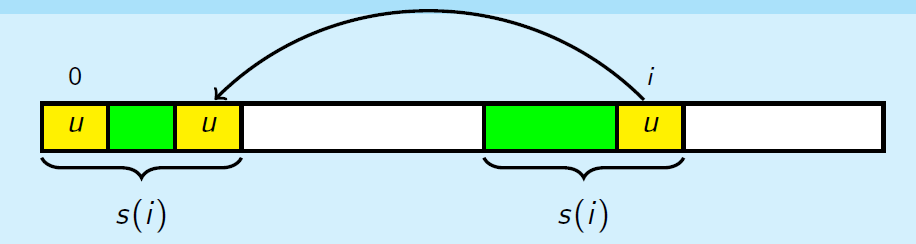
\includegraphics[width = 0.7\columnwidth]{fig/kmp_lemma_proof.png}
    \caption{Proof of Lemma}
    \label{fig:proof_border_property}
\end{figure}

For example, prefix function of string ``abcabcd'' is [0,0,0,1,2,3,0]. The trivial algorithm to implement this has $O(n^3)$ time complexity (one for loop for i, second nested for loop for k, and another n for comparing corresponding substring), which exactly follows the definition of the prefix function.  The efficient algorithm which is demonstrated to run in $O(n)$ was proposed by Knuth and Pratt and independently from them by Morris in 1977. It was used as the main function of a substring search algorithm. This is the core of Knuth Morris Pratt (KMP) algorithm. In order to implement the prefix function in linear time, we first need to utilize two properties ( facts) for the purpose of two further optimization:
\begin{enumerate}
    \item \label{observation_1} Observation: $\pi[i+1] \leq \pi[i] + 1$, which states that the value of the prefix function can either increase by one, stay the same, or decrease by some amount.
    \item \label{Lemma_1} Lemma: \textbf{If $l[i] > 0$, then all borders of P[0...i] but for the longest one are also borders of $P[0...l(i)-1]$.} The proof is: As shown in Fig.~\ref{fig:proof_border_property}, $l(i)$ is the longest border for P[0...i]. We let $\mu$ be another shorter border of P[0...i] such that $|\mu| < l(i) $. Because the first l(i) and the second is the same, this means at the first l(i), the suffix of l(i) that of the same length of $\mu$ is $\mu$. This states that $\mu$ is both a border of P[0...l(i)-1].  
 
\end{enumerate}

Now, with such knowledge we can do the following two further optimization:
\begin{enumerate}
    \item With \ref{observation_1}, the complexity can be reduced to $O(n^2)$ by getting rid of the for loop on $k$. Because each step the prefix function can grow at most one. And among all iterations of $i$, it can grow at most $n$ steps, and also only can decrease a total of $n$ steps. 
    \item With \ref{Lemma_1}, we can further get rid of the $O(n)$ string comparison each step. To accomplish this, we have to use all the information computed in the previous steps: all borders of P[0...i] (assuming it has k in total) can be enumerated from the longest to shortest as: $b_0 = \pi(i)$, $b_1 = \pi(b_0-1)$, ..., $b_{k-1} = \pi(b_{k-2}-1)$ ($b_{k-1} = 0$). Therefore, at step posited at $i+1$, instead of comparing string $s[0...\pi(i)]$ with $s[i-(\pi(i)-1)...i]$, comparison of char $s[\pi(i)]$ and $s[i]$ is needed.
\end{enumerate}



\paragraph{Implementation of Prefix Function for a Given String S} Let's recap the above optimization to get the final algorithm which computes prefix function in $O(n)$. This step is of key importance to the success of KMP algorithm. Let's understand this together with the algorithm statement and the code. 
\begin{enumerate}
    \item Initialization: assign $n$ space to $l$ array and set $l_0 = 0$. 
    \item A for loop in range of [1, m-1] to compute $l(i)$. Set a variable j = $l(i-1)$, and a while loop over j until j = 0: check if s[j] == s[i]; if true, $l(i)=j+1$, otherwise reassign j $j = l(j-1)$ in order to check smaller border.
\end{enumerate}
\begin{lstlisting}[language=Python]
def prefix_function(s):
    n = len(s)
    pi = [0] * n
    for i in range(1, n):
        # compute l(i)
        j = pi[i-1]
        while j > 0 and s[i] != s[j]: # try all borders of s[0...i-1], from the longest to the shortest
            j = pi[j-1]
        # check the character
        if s[i] == s[j]:
            pi[i] = j + 1

    return pi
\end{lstlisting}

Run an example:
\begin{lstlisting}[language=Python]
S = 'abcabcd'
print('The prefix function of: ', S, " is ", prefix_function(S))

The prefix function of:  abcabcd  is  [0, 0, 0, 1, 2, 3, 0]
\end{lstlisting}

\paragraph{Knuth Morris Pratt (KMP)} Back to the problem of eaxact pattern matching, we first build a new string as $s = P+'\$'+T$,  which is a concatenation of pattern P, '\$', and text T. Let us calculate the prefix function of string s. Now, let us think about the meaning of the prefix function, except for the first $m+1$ items (which belong to the string P and the separator '\$'): 
\begin{enumerate}
    \item For all $i$, $\pi[i] \leq m$ because of the separator '\$' in the middle of the pattern and the text that acts as a separator. 
    \item If $\pi[i] = m$, i.e. $K[0:m] = K[i-m:i] = P$. This means that the pattern P appears completely in the new string s and ends at position $i$. Now, we convert $i$ to the starting position of pattern in T with $i-2m$.
    \item If $f[i] < m$, no full occurrence of pattern ends with position i. 
\end{enumerate}

Thus the Knuth-Morris-Pratt algorithm solves the problem in $O(n+m)$ time and $O(n+m)$ memory. And can be simply implemented with prefix function as follows:
\begin{lstlisting}[language=Python]
def KMP_coarse(p, t):
    m = len(p)
    s = p + '$' + t
    n = len(s)
    pi = prefix_function(s)
    ans = []
    for i in range(2*m, n):
        if pi[i] == m:
            ans.append(i - 2*m)
    return ans
\end{lstlisting}

Because for all $\pi[i] \leq m$: for i in [0, m-1], we save the border in $\pi$; for i in [m, n+m-1], we set up a global variable $j$ to track the last border. We can decrease the space complexity in $O(m)$.
The Python implementation is given as: 
\begin{lstlisting}[language=Python]
def KMP(p, t):
    m = len(p)
    s = p + '$' + t
    n = len(s)
    pi = [0] * m
    j = pi[0]
    ans = []
    for i in range(1, n):
        # compute l(i)
        while j > 0 and s[i] != s[j]: # try all borders of s[0...i-1], from the longest to the shortest
            j = pi[j-1]
        # check the character
        if s[i] == s[j]:
            j += 1
        # record the result
        if j == m:
            ans.append(i-2*m)
        # save the result if i in [0, m-1]
        if i < m:
            pi[i] = j
    return ans
\end{lstlisting}

Run an example:
\begin{lstlisting}[language=Python]
t = 'textbooktext'
p = 'text'
print(KMP(p, t))
# output
# [0, 8]
\end{lstlisting}

\paragraph{Sliding Rule with Border Information} Now, assuming we know how to compute the border information, how do we slide instead compared with the brute force solution? There are three steps, with Fig.~\ref{fig:sliding_rule_kmp} as demonstration:

\begin{enumerate}
    \item Find longest common prefix $\mu$.
    \item Find $w$ -- the longest border of $\mu$. 
    \item Move P such that prefix $w$ in P aligns with suffix $w$ of $\mu$ in T. 
\end{enumerate}
% There exists redundant comparison between pattern and the text at different location. For example in the following case, we found a match at pos 0, if we know p[0:3]==p[1:4], then we know p[0:3]==s[1:4], in the next sliding window, s[1:5], we only need to compare if p[3]==s[4]. 
%  \begin{lstlisting}[numbers=none]
% txt = "AAAAABAAABA" 
% pat = "AAAA"  [Initial position]
%  \end{lstlisting}

% Knuth Morris Pratt is an exact pattern matching algorithm, which preprocesses the pattern string at first to recognize those patterns having same sub-patterns appearing more than once to skip characters while matching.  

% \textbf{Pattern Lookup Table.} Therefore, for the pattern we preprocess it and construct an auxiliary lookup table of size $m$ which saves the longest length of prefix before current index i which is the same as suffix. We define the table as f, we have that f[0] = 0, if f[i] = t, it means $P[:t+1] = P[i-t:i]$. The following figure(Fig~\ref{fig:lookup}) shows the example of a lookup table. 
% \begin{figure}[h]
    
%     \centering
%     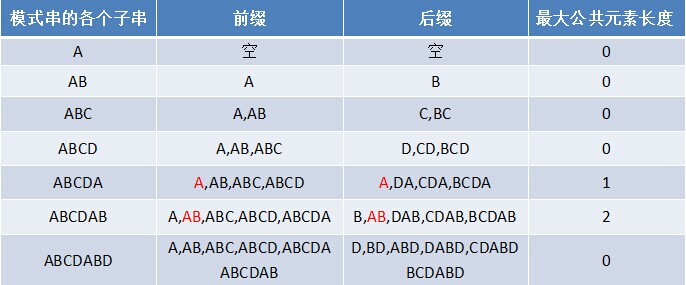
\includegraphics[width = 0.98\columnwidth]{fig/lookup.jpg}
%     \caption{The example of lookup table of KMP, which can be generated with dynamic programming.}
%     \label{fig:lookup}
    
%     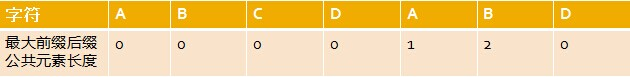
\includegraphics[width = 0.98\columnwidth]{fig/lookup_table.jpg}
%     \caption{The example of lookup table of KMP}
% \end{figure}

% \textbf{Generate Lookup Table with Dynamic Programming.} Now, we have not learn dynamic programming yet, you can come to digest this section more later. We initiate f[0]=0. At the 6th row with 'ABCDAB', we know before at 'ABCDA', the prefix 'A' matches suffix 'A', now we compare current char 'B' with the one next to prefix 'A' at position f[i-1], if it matches, then f[i] = f[i-1]+1. If it does'nt match, at 7th row, 'D' != 'C', thus we cant have 3 as the answer, we retreat to  check position f[i-2], where we have 'D'!='B', we retreat to f[i-3], and where 'A'!='D', then we have i-4 < 0, we stop, and put 0 as the result. The Python code is given as follows:
% \begin{lstlisting}[language=Python]
% def LPS(p):
%     m = len(p)
%     f = [0] * m
%     for i in range(1, m):
%         # chek the previous position
%         check_pos = f[i-1]
%         if p[i] == p[check_pos]:
%             f[i] = check_pos + 1 
%             break
%     return f
% print(LPS("ABAB"))
% print(LPS("AAABAAA"))
% # output
% # [0, 0, 1, 2]
% # [0, 1, 2, 0, 1, 2, 3]
% \end{lstlisting}

% \begin{lstlisting}[language = Python]
% # Generating lookup table for string S using Python
% f=[0]*n
% for i in xrange(1,n):
%     t = f[i-1]
%     while t > 0 and S[i] != S[t]:
%         t = f[t-1]
%     if S[i] == S[t]:
%         t +=1 
%     f[i] = t
% \end{lstlisting}
\paragraph{Knuth Morris Pratt $O(m+n)$} Now, to complete the picture of KMP, when we have the lookup table at hand, when we failed to match i and j, we set j = lps[j-1], and i doest not need to backtrack.
\begin{lstlisting}[language = Python]
def KMP(p, ps):
    f = LPS(p)
    n =m, n = len(p), len(ts)

    i = 0 # index in s
    j = 0 # index in p
    pos = []
    while i < n:
        if p[j] == s[i]:
            i += 1 
            posj += 1 
            dp[i] = pos
            if dp[i] == m:if j == m: # i at i+1, j at f[j-1]
                print("Found pattern at index ", i-j) 
                ans.append(i-2*mj)
            i += 1
        else:
            if pos > 0:    j = f[j-1] 
        else: # mismatch at i and j 
            if j != 0: # if j can retreat with lps, then i keep the same
                pos = dp[posj = f[j-1]
            else:
                i += 1 #the value is 0
    return ans # if j needs to start over, i moves too 
                i += 1
    return ans
print(KMP(p,s))
# [0, 9, 12]
\end{lstlisting}

%%%%%%%%%%%%%%%%%%%%%%Application of Prefix Function
\subsection{More Applications of Prefix Functions}


\paragraph{Counting the number of occurrences of each prefix}

\paragraph{Counting the number of occurrences of different substring in a string}

\paragraph{Compressing a string}

% \paragraph{}


%%%%%%%%%%%%%%%%%%%%%%%Z-function%%%%%%%%%%%
\subsection{Z-function} 
\subsubsection{Definition and Implementation}
Z-function for a string $s$ of length $n$ is defined as an array $z[i] = k, i \in [1, n-1]$. At item $z[i]=k$ stores the longest substring starting at index $i$ which is also a prefix of string $s$. To notice, the length of the substring has to be smaller than the whole length, therefore, $z[0]=0$.  In other words, it means the  the length of the longest common prefix between $s$ and substring $s[i:n]$. %Thus, $z[i]=k$  tells us that $s[0...k-1] = s[i...i+k−1]$. 
For example:
\begin{lstlisting}[numbers=none]
"aaaaa" - [0,4,3,2,1]
a
a substring 'aaaa' = prefix 'aaaa'
a substring 'aaa' = prefix 'aaa'
a substring 'aa' = prefix 'aa'
a substring 'a' = prefix 'a'
\end{lstlisting}
Another Example.
\begin{lstlisting}[numbers=none]
"aaabaab" - [0,2,1,0,2,1,0]
a  0 
a  substring 'aa' = prefix 'aa'
a  substring 'a' = prefix 'a'
b  0
a  substring 'aa' = prefix 'aa'
a  substring 'a' = prefix 'a'
b  
\end{lstlisting}
z-function can be represented with a formula:
\begin{equation}
    l[i] = \max_{k=0,...,i}\{k+1: P[0...k] = P[i...i+k]\}
\end{equation}
The naive implementation of  z-function takes $O(n^2)$ time complexity just as the prefix function. 
\begin{lstlisting}[language=Python]
def naiveZF(s):
  n = len(s)
  z = [0] * n
  for i in range(1, n): # starting point
    k = 0
    while i + k < n and s[i + k] == s[k]:
      k += 1
    z[i] = k
  return z
\end{lstlisting}
\paragraph{Z-function Property}
Here, we show how we can implement it in $O(n)$. To compute $z[i]$, do we have to start at $i$, then follows the order of $i+1$, $i+2$, ..., $i+k$? The answer is No.
\begin{figure}[h]
    \centering
    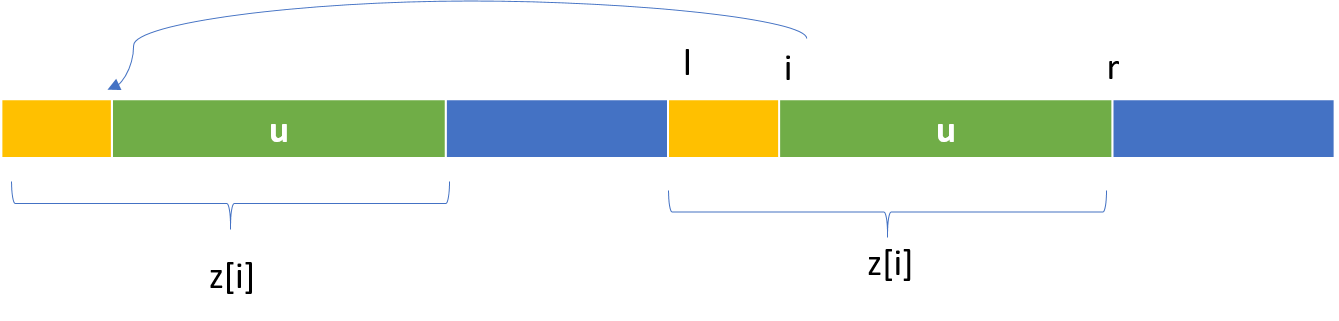
\includegraphics[width = 0.9\columnwidth]{fig/z_function.png}
    \caption{Z function property}
    \label{fig:z_function_property}
\end{figure}
First, As shown in Fig.~\ref{fig:z_function_property}, for a given position $i$,  $[l, r]$ is one of its preceding non-zero $z[p], p< i$, which has the furthest right boundary $r$. We can think it as a rightmost window, wherein $s[l, r] = s[0, r-l+1]$.  $s[0, i-l]$ is marked as yellow. We divide the area in range $[0, r-l+1]$ into yellow $[0, l-i]$ and a green parts $[l-i+1, r-l+1]$. Therefore, to compare range $[i, r]$ with prefix is the same as of comparing range $[l-i+1, r-l+1]$ with the prefix, which already has a result $z[i-l]$. So instead, our $k$ can start from position $z[i-l]$. However, there are two more restrictions:
\begin{enumerate}
    \item Enable to utilize z-function property, $r \geq i$ because the index $r$ can be seen as ``boundary'' to which our string $s$ has been scanned by the algorithm. 
    \item The initial approximation for $z[i]$ is bounded by the length between $r$ and $i$, which is $r-i+1$. Therefore, we modify our initial approximation to $z[i]$ to $z[i] = \min(r-i+1, z[i-l])$ instead.
\end{enumerate}

Now, the $O(n)$ implementation is given as follows:
\begin{lstlisting}[language=Python]
def linearZF(s):
  n = len(s)
  z = [0] * n
  l = r = 0
  for i in range(1, n): 
    k = 0
    if i <= r: # r is the right bound has been scanned
      k = min(r-i+1, z[i - l])
    while i + k < n and s[i+k] == s[k]:
      k += 1
    # update the boundary
    if i + k - 1 > r:
      l = i
      r = i + k - 1 
    z[i] = k 
  return z
\end{lstlisting}

\subsubsection{Applications}
The applications of Z-function are largely similar to those of prefix function. Therefore, the applications will be explained briefly compared with the applications of prefix functions. If you have problems to understand this section, please read the prefix function first.

\paragraph{Exact Single-Pattern Matching} In this problem set, we are asked to find all occurrences of the pattern $p$ inside the text $t$. We can do the same as of in the KMP, we create a new string $s=p+\$+t$. Then, we compute the z-function for $s$. With the z array, for $z[i]=k$, if $k=|p|$, then we know there is one occurrence of p starting in the i-th position in $s$, which is $i-(|p|+1)$ in the t. 
\begin{lstlisting}[language=Python]
def findPattern(p, t):
  s = p + '$' + t
  m = len(p)
  z = (linearZF(s))
  ans = []
  for i, v in enumerate(z):
    if v == m:
      ans.append(i-m-1)
  return ans
\end{lstlisting}

\paragraph{Number of distinct substrings in a string} Given a string s of length n, count the number of distinct substrings of s. 

To solve this problem we need to use dynamic programming and the subproblems are $s[0...0]$, $s[0...1]$, ..., $s[1...i]$,...$s[0...n-1]$. For example, given ``abc'', 
\begin{lstlisting}[numbers=none]
subproblem 1: 'a', dp[0] = 1
subproblem 2: 'ab', dp[1] = 2, with new substrings 'b', 'ab'
subproblem 3, 'abc', dp[2] = 3, new substrs 'c', 'bc', 'abc'
\end{lstlisting}

We know the maximum for dp[i] is $i+1$, however for cases like ``aaa''', the situation is different:
\begin{lstlisting}[numbers=none]
subproblem 1: 'a', dp[0] = 1
subproblem 2: 'aa', dp[1] = 1, 'aa', because 'a'_1 == 'a_0'
subproblem 3, 'aaa', dp[2] = 1, new substrs 'aaa', because 'a_0a_1'='a_1a_2', 'a_2' = 'a_0'. 
\end{lstlisting}

If for each subproblem i, we take the string s[0...i] and reverse it $i...0$. If using z-function on this substring, we can find the number of prefixes of the reversed string are found somewhere else in it, which is the maximum value of its z-function.  This is because if we know z[j] = max(k), then s[i...i-max-1] = s[i-j...i-j+max], which is to say s[i-max-1...i] = s[i-j-max...i-j]
With the max value, all of the shorter prefixes also occur too. Therefore, $dp[i] = i+1 - max(z[i])$. The time complexity is $O(n^2)$
\begin{lstlisting}[language=Python]
def distinctSubstrs(s):
  n = len(s)
  if n < 1:
    return 0
  ans = 1 # for dp[0]
  #last_str = s[0:1]
  for i in range(1, n):
    reverse_str = s[0:i+1][::-1]
    z = linearZF(reverse_str)
    ans += (i + 1 - max(z))
  return ans
\end{lstlisting}

Run an example:
\begin{lstlisting}[language=Python]
s = 'abab'
print(distinctSubstrs(s))
# output
# 7
\end{lstlisting}

\section{Exact Multi-Patterns Matching}

%%%%%%%%%%%%%%%%%%%%%%%%%%%%%%%%%%%%%%%%%%%%%%%%%%%%%%%%%%%%%%%%%%%%%%%%%%%
%%%%% Rabin-Karp algorithm
%%%%%%%%%%%%%%%%%%%%%%%%%%%%%%%%%%%%%%%%%%%%%%%%%%%%%%%%%%%%%%%%%%%%%%%%%%%
\subsection{Suffix Trie/Tree/Array Introduction}
\label{pattern_matching_subsec_suffix_trie}
Up till now, prefix function and the KMP algorithms seems impeccable with its liner time and space complexity. However, there are two problems that KMP can not resolve:
\begin{enumerate}
    \item Approximate matching, which we will detail more in the next section.
    \item If frequent queries will be made on the same text with a given pattern, and if the $m<<n$, then KMP become impractical.
\end{enumerate}

The solution to the second problem of KMP is preprocess the text and store it in order to obtain an algorithm with time complexity only related to the length of the pattern for each query. Building a suffix trie of the text is such a solution. 

\paragraph{Suffix Trie} A suffix trie of a given string is defined as: 

\paragraph{Suffix Tree} If we compress the above suffix trie, we get suffix tree. 

\paragraph{Suffix Array} Suffix Array is further applied with the benefits of saving space in storage. 

\paragraph{Suffix Tree VS Suffix Array} Each data structure has its own pros and cons. In reality, conversion between these two can be implemented in $O(n)$ time. Therefore, we can first construct one and convert it to the other later. 

\subsection{Suffix Array and Pattern Matching}
\label{pattern_matching_subsec_suffix_array}
\subsubsection{Definition and Implementation}
Suffix Array of a given string s is defined as all suffixes of this string in lexicographical order. Because no any two suffixes can have the same length, thus the sorting will not have equal items. For example, given s = 'ababaa', the suffix array will be:
\begin{lstlisting}[numbers=none]
'a'
'aa'
'abaa'
'ababaa'
'baa'
'babaa'
\end{lstlisting}

To avoid the prefix rule defined in the lexicographical order, as shown with example 'ab' < 'abab', we append a special character '\$' at the end of all suffixes. '\$' is smaller than all other characters. With this operation, we have 'ab\$' and 'abab\$'. At position 2, '\$' will be smaller than 'a' or any other character and 'ab\$' is still smaller than 'abab\$'. Therefore, adding this special character will not lead to different sorting result, and can avoid the prefix rule when comparing two different strings. 

\paragraph{Naive Solution with $O(n^2\log n)$ time complexity} With this knowledge, we get s = s + '\$', and we can generate the suffix array and sort them. A stable sorting algorithm takes $O(n\log n)$ comparison, and each comparison takes additional $O(n)$, which makes the total time complexity of $O(n^2\log n)$. 
\begin{lstlisting}[language=Python]
def generateSuffixArray(s):
    s = s + '$'
    n = len(s)
    suffixArray = [None]*n
    # generate
    for i in range(n):
        suffixArray[i] = s[i:]
    #print(suffixArray)
    suffixArray.sort()
    print(suffixArray)
    # save space by storing the order of the suffixes, which is the starting index
    for idx, suffix in enumerate(suffixArray):
         suffixArray[idx] = n - len(suffix)
    print(suffixArray)
    return suffixArray
\end{lstlisting}

Run the above example, we will have the following output:
\begin{lstlisting}[numbers=none]
['$', 'a$', 'aa$', 'abaa$', 'ababaa$', 'baa$', 'babaa$']
[6, 5, 4, 2, 0, 3, 1]
\end{lstlisting}

\begin{figure}[h]
    \centering
    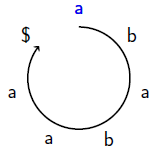
\includegraphics[width = 0.5\columnwidth]{fig/cyclic_shift.png}
    \caption{Cyclic Shifts}
    \label{fig:clyclic_shifts}
\end{figure}
\paragraph{Cyclic Shifts} For our example, we start at position 0, we get the first cyclic shift of 'ababaa\$', and then position 1, we have our second cyclic shift 'babaa\$a', and so till the last position of the string. Now, let us see what happens if we sort all of the cyclic shifts:
\begin{lstlisting}[numbers=none]
             Sorted    To Suffix Array
0:ababaa$    $ababaa    $
1:babaa$a    a$ababa    a$
2:abaa$ab    aa$abab    aa$
3:baa$aba    abaa$ab    abaa$
4:aa$abab    ababaa$    ababaa$
5:a$ababa    baa$aba    baa$
6:$ababaa    babaa$a    babaa$
\end{lstlisting}

We know the number of cyclic shifts is the same as of the number of all suffixes of the same string. And by observing the above example, sorting the cyclic shifts will get us sorted suffixes if we remove all characters after '\$' in each cyclic shift. This conclusion can be hold true for all strings because '\$' is smaller than all other characters, and with '\$' at different position in each cyclic shift, once we are at '\$', the comparison of two strings end because the first one that has '\$' is smaller than all others. Therefore, all the characters after the '\$' will not affect the sorting at all. Now, we know that sorting cyclic shifts and suffixes of string s is equivalent with the addition of '\$' at the end. 

If we can sort the cyclic shifts of string in faster way, then we will find ourselves a more efficient suffix sorting algorithm. One obvious efficient sorting algorithm is using Radix Sort. Using radix sort, we first sort the cyclic shifts by the last character using counting sort, and then the second last character till finishing the first character. Sorting each character for the whole cyclic shifts array takes $O(n)$, and we are running $n$ rounds, this makes the whole sorting of $O(n^2)$ and with $O(n)$ space. However, we can improve these complexity further by using special properties of the Cyclic shifts. %Before we give out the eventual algorithm and implementation, let us learn more concepts to help out later.

\paragraph{Partial Cyclic Shifts} Different from the cyclic shifts, partial cyclic shifts are defined as $C^{L}_i$ which is the partial cyclic shift of length $L$ starting at index $i$. For the above example, the partial cyclic shift of length 1, 2, and 4 will be :
\begin{lstlisting}[numbers=none,mathescape=true, escapechar=\%]
  $C^7$      $C^1$   $C^2$    $C^4$
ababaa%\$%    a    a%\underline{b}%    ab%\underline{ab}%
babaa%\$%a    b    b%\underline{a}%    ba%\underline{ba}%
abaa%\$%ab    a    a%\underline{b}%    ab%\underline{aa}%
baa%\$%aba    b    b%\underline{a}%    ba%\underline{a\$}%
aa%\$%abab    a    a%\underline{a}%    aa%\underline{\$a}%
a%\$%ababa    a    a%\underline{\$}%    a%\$\underline{ba}%
%\$%ababaa    %\$%    %\$\underline{a}%    %\$a\underline{ba}%
\end{lstlisting}
Carefully observing the relation of pair $(C_1, C_2)$ and $(C_2, C_4)$. We can find that $C_1$ and the second half of substring (denoted by underline) in $C_2$ has the same key set. Same rule applies to $C_2$ and the second half of substring in $C_4$.

\paragraph{Doubled Partial Cyclic Shifts} \textit{Doubled Partial Cyclic Shifts} of $C^L_i$ is $C^{2L}_i$ and $C^{2L}_i = C^{L}_iC^{L}_{i+L}$ (with concatenation of these two strings). Apply the same methodology of Radix Sort, we can sort the doubled partial shifts by firstly sort the second half and then the first half. Therefore, instead of doing $n$ rounds of counting sort on each character, we do $\log n$ rounds of sorting of the doubled partial cyclic shifts from the last round. If we can sort each round in $O(n)$, then we make the time complexity to $O(n \log)$ ($T(n) = T(n/2)$) which is way better than the radix sort of $O(n^2)$.  The starting point of sorting doubled partial cyclic is sorting the partial cyclic shifts with length one. 

\paragraph{Order and Class} \textit{Order} is defined as the sorted cyclic shift with the starting index as their value. For example, for $C^1$, the sorted order will be $[6, 0, 2, 4, 5, 1, 3]$, which represents $[\$, a, a, a, a, b, b]$. \textit{Class} is an array that each item $Class_{i}$ corresponds to $C_i$ and denotes as the number of partial cyclic shifts of the same length that are strictly smaller than $C_i$. For 'ababaa\$', the class of length 1 will be $[1, 2, 1, 2, 1, 1, 0]$. The reason to bring in the concept of class is because of the rule that the set of first and second half of the doubled partial cyclic shifts share the same key set, and \textbf{the class is equivalent to the converted key of corresponding partial cyclic shift}. 

\paragraph{Compute Order and Class of Partial Cyclic Shifts of Length 1} For $C^1$: , we can obtain with counting sort with the range of 256 for all common English characters.  For $C^1$,  we know for $[\$, a, a, a, a, b, b]$, we assign order as $[0, 1, 1, 1, 1, 2, 2]$. Each one corresponds to $C_{order_i}$.  Because the class corresponds to the original string order, therefore, we just need to put these class back to $order_i$ position in the array. We recap this as: we first set $class[order[0]] = 0$, and looping over the order array from [1, n-1], the corresponding character will be $s[order[i]$ and the last order char will be $s[order[i-1]]$.  We just need to compare if it equals.
\begin{lstlisting}[numbers=none]
if s[order[i]] != s[order[i-1]]:
    # use order as index to put the result back
    class[order[i]] = class[order[i-1]] + 1
else:
    class[order[i]] = class[order[i-1]]
\end{lstlisting}

The Python implementation  of Computing Order for Partial Cyclic Shift of Length 1, the time complexity is $O(n+k)$, $k$ is the number of possible characters. 
\begin{lstlisting}[language=Python]
def getCharOrder(s):
  n = len(s)
  numChars = 256
  count = [0]*numChars # totally 256 chars, if you want, can print it out to see these chars
  
  order = [0]*(n)
  
  #count the occurrence of each char
  for c in s:
    count[ord(c)] += 1
    
  # prefix sum of each char
  for i in range(1, numChars):
    count[i] += count[i-1]
    
  # assign from count down to be stable
  for i in range(n-1,-1,-1):
    count[ord(s[i])] -=1
    order[count[ord(s[i])]] = i # put the index into the order instead the suffix string
    
  return order
\end{lstlisting}

The Python implementation  of Computing Class for Partial Cyclic Shift of Length 1, this can be applied in $O(n)$ given the order. 
\begin{lstlisting}[language=Python]
def getCharClass(s, order):
  n = len(s)
  cls = [0]*n
  # if it all differs, then cls[i] = order[i]
  cls[order[0]] = 0 #the 6th will be 0
  for i in range(1, n):
    # use order[i] as index, so the last index
    if s[order[i]] != s[order[i-1]]:
      print('diff',s[order[i]],s[order[i-1]])
      cls[order[i]] = cls[order[i-1]] + 1
    else:
      cls[order[i]] = cls[order[i-1]]
  return cls
\end{lstlisting}

Applying the above two functions, we can get:
\begin{lstlisting}[numbers=none]
   L=1 cls order    CL=2  order cls
i=0, a:1    $:6     a$:5  $a:6  ab:3
i=1, b:2    a:0     $a:6  a$:5  ba:4
i=2, a:1    a:2     ba:1  aa:4  ab:3
i=3, b:2    a:4     ba:3  ab:0  ba:4
i=4, a:1    a:5     aa:4  ab:2  aa:2
i=5, a:1    b:1     ab:0  ba:1  a$:1
i=6, $:0    b:3     ab:2  ba:3  $a:0
\end{lstlisting}

\paragraph{Sort the Doubled Partial Cyclic shifts} To apply radix sorting, we double our previous sorted partial shifts of $C^L_i$ as $C^{L}_{i-L}C^{L}_{i}$. Given the fact that the second part $C^{L}_{i}$ is already sorted, we just need to sort the first half with counting sort using the class array of the last partial cyclic shifts. The time complexity of this step is $O(n)$ too. The Python implementation of computing the doubled partial cyclic shifts' order is:
\begin{lstlisting}[language=Python]
'''It is a counting sort using the first part as class'''
def sortDoubled(s, L, order, cls):
  n = len(s)
  count = [0] * n
  new_order = [0] * n
  # their key is the class
  for i in range(n):
    count[cls[i]] += 1
    
  # prefix sum
  for i in range(1, n):
    count[i] += count[i-1]
    
  # assign from count down to be stable
  # sort the first half
  for i in range(n-1, -1, -1):
    start = (order[i] - L + n) % n #get the start index of the first half, 
    count[cls[start]] -= 1
    new_order[count[cls[start]]] = start
    
  return new_order
\end{lstlisting}

Now, similarily, we compute the new class information. The comparison of the string is converted to compare its corresponding class info, as a pair $(P_1, P_2)$ which is the class of the first and second half. 
\begin{lstlisting}[language=Python]
def updateClass(order, cls, L):
  n = len(order)
  new_cls = [0]*n
  # if it all differs, then cls[i] = order[i]
  new_cls[order[0]] = 0 #the 6th will be 0
  for i in range(1, n):
    cur_order, prev_order = order[i], order[i-1]
    # use order[i] as index, so the last index
    if cls[cur_order] != cls[prev_order] or cls[(cur_order+L) % n] != cls[(prev_order+L) % n]:
      new_cls[cur_order] = new_cls[prev_order] + 1
    else:
      new_cls[cur_order] = new_cls[prev_order]
  return new_cls
\end{lstlisting}


\paragraph{Sorting Cyclic Shifts in $O(n\log n)$}  Now, we have derived ourselves a $O(n\log n)$ suffix array construction algorithm. We start from sorting partial cyclic shifts of length 1 and each time to double the length untill the the sorted length is >= to the string's length.

\begin{lstlisting}[language=Python]
def cyclic_shifts_sort(s):
  s = s + '$'
  n = len(s)
  order = getCharOrder(s)
  cls = getCharClass(s, order)
  print(order, cls)
  L = 1
  while L < n:
    order = sortDoubled(s, 1, order, cls)
    cls = updateClass(order, cls, L)
    print(order, cls)
    L *= 2
  
  return order
\end{lstlisting}

\subsubsection{Applications}
\paragraph{Number of Distinct Substrings of a string}
%%%%%%%%%%%%%%%%%%%%%%%%%%%%%%%%%%%%%%%%%%%%%%%%%%%%%%%%%%%%%%%%%%%%%%%%%%%
%%%%% Rabin-Karp algorithm
%%%%%%%%%%%%%%%%%%%%%%%%%%%%%%%%%%%%%%%%%%%%%%%%%%%%%%%%%%%%%%%%%%%%%%%%%%%
\subsection{Rabin-Karp Algorithm (Exact or anagram Pattern Matching) }
Used to find the exact pattern, because different anagram of string would have different hash value.

%%%%%%%%%%%%%%%%%%%%%%%%%%%%%%%%%%%%%%%%%%%%%%%%%%%%%%%%%%%%%%%%%%%%%%%%%%%
%%%%% Bonus
%%%%%%%%%%%%%%%%%%%%%%%%%%%%%%%%%%%%%%%%%%%%%%%%%%%%%%%%%%%%%%%%%%%%%%%%%%%
\section{Bonus}


\begin{figure}[h]
    \centering
    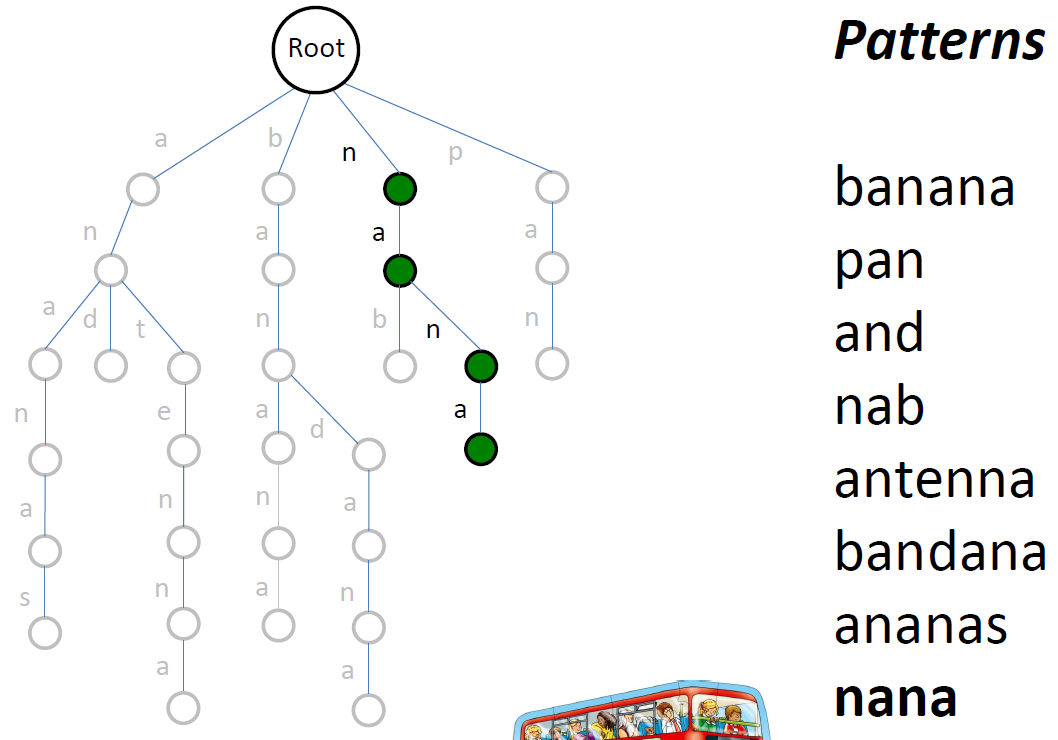
\includegraphics[width = 0.7\columnwidth]{fig/trie_pattern.png}
    \caption{Building a Trie from Patterns}
    \label{fig:trie_pattern}
\end{figure}
\paragraph{Multiple-Patterns Matching} Previously, we mainly talked about exact/approximate one pattern matching. When there are multiple patterns the time complexity became to $O(\sum_i{m_i*n})$ if brute force solution is used. We can construct a trie of all patterns as shown in Section~\ref{concept_trie}. For example, in Fig.~\ref{fig:trie_pattern} shows a trie built with all patterns. 

Now, let us do \textbf{Trie Matching} exactly the same way as the brute force pattern matching algorithm by sliding the pattern trie along the text at each position of text. Each comparison: walk down the trie by spelling symbols of text and a pattern from the pattern list matches text each time we reach a leaf. Try text = ``panamabananas''. We will first walk down branch of p->a->n and stop at the leaf, thus we find pattern `pan`. With Trie Matching, the runtime is decreased to $O(\max_i{m_i*n})$. Plus the trie construction time $O(\sum_i{m_i})$. 

However, merging all patterns into a trie makes it impossible for using advanced single-pattern matching algorithms such as KMP. 

\paragraph{More Pattern Matching Tasks} There are more types of matching, instead of finding the exact occurrence of one string in another.
\begin{enumerate}
    \item Longest Common Substring (LCS): LCS asks us to return the longest substring between these two strings.
    \item Anagram Matching: this asks us to find a substring in T that has all letters in P, and does not care about the order of these letters in P.
    \item Palindrome Matching.
\end{enumerate}

%%%%%%%%%%%%%%%%%%%Trie%%%%%%%%%%%%%%%%%
\section{Trie for String}
\label{concept_trie}
\paragraph{Definition} Trie comes from the word re\textbf{Trie}val. In computer science, a trie, also called digital tree, radix tree or prefix tree which like BST is also a kind of search tree for finding substring in a text. We can solve string matching in $O(|T|)$ time,  where |T| is the size of our text.  This purely algorithmic approach has been studied extensively in the algorithms:  Knuth-Morris-Pratt, Boyer-Moore, and Rabin-Karp. However, we entertain the possibility that multiple queries will be made to the same text.  This motivates the development of data structures that preprocess the text to allow for more efficient queries. Such efficient data structure is Trie, which can do each query in $O(P)$, where P is the length of the pattern string. Trie is an ordered tree structure, which is used mostly for storing strings (like words in dictionary) in a compact way. 
\begin{enumerate}
    \item In a Trie, each child branch is labeled with letters in the alphabet $\sum$. Actually, it is not necessary to store the letter as the key, because if we  order the child branches of every node alphabetically from left to right, the position in the tree defines the key which it is associated to. 
    \item The root node in a Trie represents an empty string. 
\end{enumerate}
% An ordered tree data structure used to store a dynamic set or associative array where the keys are usually strings. Unlike a binary search tree, no node in the tree stores the key associated with that node; instead, its position in the tree defines the key with which it is associated. 

Now, we define a trie Node: first it would have a bool variable to denote if it is the end of the word and a children which is a list of of 26 children TrieNodes. 
\begin{lstlisting}[language= Python]
class TrieNode:
    # Trie node class
    def __init__(self):
        self.children = [None]*26
        # isEndOfWord is True if node represent the end of the word
        self.isEndOfWord = False
\end{lstlisting}
\begin{figure}[h]
    \centering
    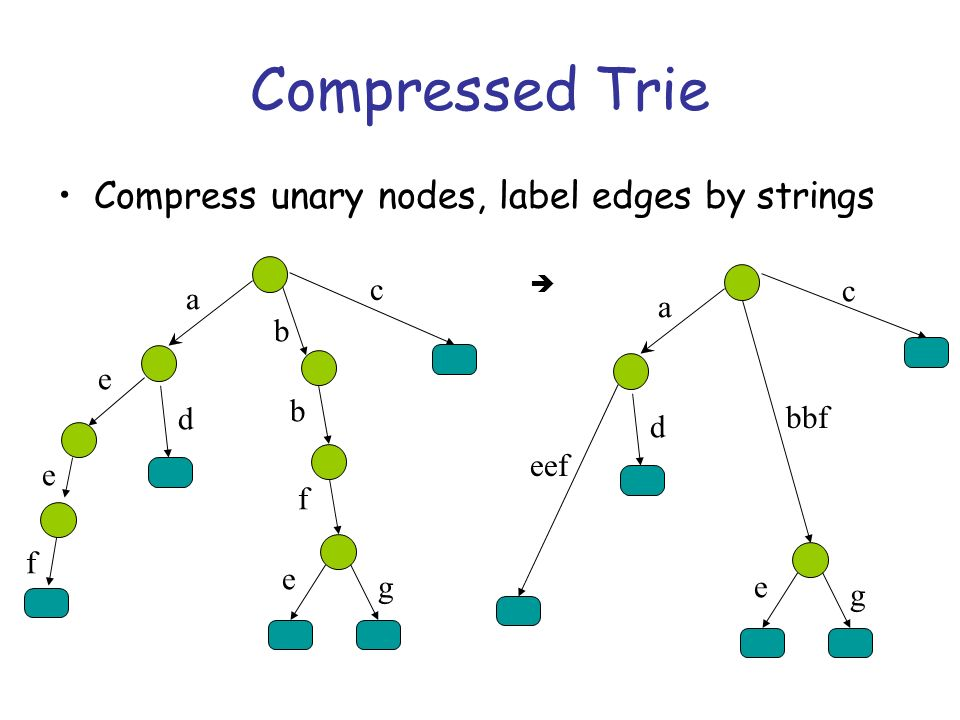
\includegraphics[width=0.6\columnwidth]{fig/trie_compact_trie.jpg}
    \caption{Trie VS Compact Trie}
    \label{fig:trie_compact_trie}
\end{figure}

\paragraph{Compact Trie} If we assign only one letter per edge, we are not taking full advantage of the trie’s tree structure. It is more useful to consider compact or compressed tries, tries where we remove the one letter per edge constraint, and contract non-branching paths by concatenating the letters on these paths.
In this way, every node branches out, and every node traversed represents a choice between two different words.  The compressed trie that corresponds to our example trie is also shown in Figure
~\ref{fig:trie_compact_trie}. 

\paragraph{Operations: INSERT, SEARCH}
% Now, let us solve an LeetCode problem together which requires us to implement a complete Trie that with the operations INSERT, SEARCH, STARTWITH. All of these operations are actually quickly similar and they all require us to simultaneously iterate each character in the input string (or word) and each level of the Trie on the location of that character. So, it would not be hard to get the worst time complexity when we searched the whole tree or finished iterating the characters in the input. 
Both for INSERT and SEARCH, it takes $O(m)$, where m is the length of the word/string we wand to insert or search in the trie. Here, we use an LeetCode problem as an example showing how to implement INSERT and SEARCH. Because constructing a trie is a series of INSERT operations which will take $O(n*m)$, n is the total numbers of words/strings, and m is the average length of each item. The space complexity fof the non-compact Trie would be $O(N*|\sum|)$, where $|\sum|$ is the alphlbetical size, and N is the total number of nodes in the trie structure. The upper bound of N is $n*m$. 
\begin{figure}[h]
    \centering
    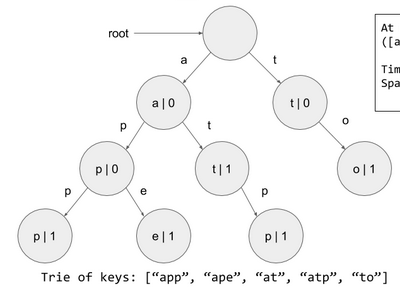
\includegraphics[width=0.6\columnwidth]{fig/Trie.png}
    \caption{Trie Structure}
    \label{fig:trie}
\end{figure}
\begin{examples}
\item \textbf{208. Implement Trie (Prefix Tree) (medium).} Implement a trie with insert, search, and startsWith methods.
\begin{lstlisting}
Example:
Trie trie = new Trie();
trie.insert("apple");
trie.search("apple");   // returns true
trie.search("app");     // returns false
trie.startsWith("app"); // returns true
trie.insert("app");   
trie.search("app");     // returns true
\end{lstlisting}
\textit{Note: You may assume that all inputs are consist of lowercase letters a-z. All inputs are guaranteed to be non-empty strings.}

\paragraph{INSERT} with INSERT operation, we woould be able to insert a given word in the trie, when traversing the trie from the root node which is a TrieNode, with each letter in world, if its corresponding node is None, we need to put a node, and continue. At the end, we need to set that node's endofWord variable to True. thereafter, we would have a new branch starts from that node constructured. For example, when we first insert ``app`` as shown in Fig~\ref{fig:trie_compact_trie}, we would end up building branch ``app``, and with ape, we would add nodes ``e`` as demonstrated with red arrows. 
\begin{lstlisting}[language=Python]
def insert(self, word):
    """
    Inserts a word into the trie.
    :type word: str
    :rtype: void
    """
    node = self.root #start from the root node
    for c in word:
        loc = ord(c)-ord('a')
        if node.children[loc] is  None: # char does not exist, new one
            node.children[loc] = self.TrieNode()
        # move to the next node
        node = node.children[loc]
    # set the flag to true
    node.is_word = True 
\end{lstlisting}

\paragraph{SEARCH} For SEARCH, like INSERT, we traverse the trie using the letters as pointers to the next branch. There are three cases: 1) for word P, if it doesnt exist, but its prefix does exist, then we return False. 2) If we found a matching for all the letters of P, at the last node, we need to check if it is a leaf node where is\_word is True.  STARTWITH is just slightly different from SEARCH, it does not need to check that and return True after all letters matched. 
\begin{lstlisting}[language=Python]
def search(self, word):
    node = self.root
    for c in word:
        loc = ord(c)-ord('a')
        # case 1: not all letters matched 
        if node.children[loc] is None: 
            return False          
        node = node.children[loc]
    # case 2
    return True if node.is_word else False
\end{lstlisting}
\begin{lstlisting}[language=Python]
def startWith(self, word):
    node = self.root
    for c in word:
        loc = ord(c)-ord('a')
        # case 1: not all letters matched 
        if node.children[loc] is None: 
            return False          
        node = node.children[loc]
    # case 2
    return True
\end{lstlisting}
Now complete the given Trie class with TrieNode and \_\_init\_\_ function.
\begin{lstlisting}[language=Python]
class Trie:
    class TrieNode:
        def __init__(self):
            self.is_word = False
            self.children = [None] * 26 #the order of the node represents a char

    def __init__(self):
        """
        Initialize your data structure here.
        """
        self.root = self.TrieNode() # root has value None       
\end{lstlisting}
\end{examples}

\begin{examples}
\item \textbf{336. Palindrome Pairs (hard).} Given a list of unique words, find all pairs of distinct indices (i, j) in the given list, so that the concatenation of the two words, i.e. words[i] + words[j] is a palindrome.
\begin{lstlisting}
Example 1:

Input: ["abcd","dcba","lls","s","sssll"]
Output: [[0,1],[1,0],[3,2],[2,4]] 
Explanation: The palindromes are ["dcbaabcd","abcddcba","slls","llssssll"]

Example 2:

Input: ["bat","tab","cat"]
Output: [[0,1],[1,0]] 
Explanation: The palindromes are ["battab","tabbat"]
\end{lstlisting}
\textbf{Solution: One Forward Trie and Another Backward Trie.}  We start from the naive solution, which means for each element, we check if it is palindrome with all the other strings. And from the example 1, [3,3] can be a pair, but it is not one of the outputs, which means this is a combination problem, the time complexity is ${C_n}{C_{n-1}}$, and multiply it with the average length of all the strings, we make it $m$, which makes the complexity to be $O(mn^2)$. However, we can use Trie Structure, 
\begin{lstlisting}[language = Python]
from collections import defaultdict


class Trie:
    def __init__(self):
        self.links = defaultdict(self.__class__)
        self.index = None
        # holds indices which contain this prefix and whose remainder is a palindrome
        self.pali_indices = set()

    def insert(self, word, i):
        trie = self
        for j, ch in enumerate(word):
            trie = trie.links[ch]
            if word[j+1:] and is_palindrome(word[j+1:]):
                trie.pali_indices.add(i)
        trie.index = i


def is_palindrome(word):
    i, j = 0, len(word) - 1
    while i <= j:
        if word[i] != word[j]:
            return False
        i += 1
        j -= 1
    return True


class Solution:
    def palindromePairs(self, words):
        '''Find pairs of palindromes in O(n*k^2) time and O(n*k) space.'''
        root = Trie()
        res = []
        for i, word in enumerate(words):
            if not word:
                continue
            root.insert(word[::-1], i)
        for i, word in enumerate(words):
            if not word:
                continue
            trie = root
            for j, ch in enumerate(word):
                if ch not in trie.links:
                    break
                trie = trie.links[ch]
                if is_palindrome(word[j+1:]) and trie.index is not None and trie.index != i:
                    # if this word completes to a palindrome and the prefix is a word, complete it
                    res.append([i, trie.index])
            else:
                # this word is a reverse suffix of other words, combine with those that complete to a palindrome
                for pali_index in trie.pali_indices:
                    if i != pali_index:
                        res.append([i, pali_index])
        if '' in words:
            j = words.index('')
            for i, word in enumerate(words):
                if i != j and is_palindrome(word):
                    res.append([i, j])
                    res.append([j, i])
        return res
\end{lstlisting}
\textbf{Solution2: .}Moreover, there are always more clever ways to solve these problems. Let us look at a clever way:
 abcd, the prefix is ''. 'a', 'ab', 'abc', 'abcd', if the prefix is a palindrome, so the reverse[abcd], reverse[dc], to find them in the words, the words stored in the words with index is fastest to find. $O(n)$. Note that when considering suffixes, we explicitly leave out the empty string to avoid counting duplicates. That is, if a palindrome can be created by appending an entire other word to the current word, then we will already consider such a palindrome when considering the empty string as prefix for the other word.
 \begin{lstlisting}[language = Python]
 class Solution(object):
    def palindromePairs(self, words):
        # 0 means the word is not reversed, 1 means the word is reversed
        words, length, result = sorted([(w, 0, i, len(w)) for i, w in enumerate(words)] +
                                   [(w[::-1], 1, i, len(w)) for i, w in enumerate(words)]), len(words) * 2, []

        #after the sorting,the same string were nearby, one is 0 and one is 1
        for i, (word1, rev1, ind1, len1) in enumerate(words):
            for j in xrange(i + 1, length):
                word2, rev2, ind2, _ = words[j]
                #print word1, word2
                if word2.startswith(word1): # word2 might be longer 
                    if ind1 != ind2 and rev1 ^ rev2: # one is reversed one is not
                        rest = word2[len1:]
                        if rest == rest[::-1]: result += ([ind1, ind2],) if rev2 else ([ind2, ind1],) # if rev2 is reversed, the from ind1 to ind2
                else:
                    break # from the point of view, break is powerful, this way, we only deal with possible reversed, 
        return result
 \end{lstlisting}
 \end{examples}
 
 %https://fizzbuzzed.com/top-interview-questions-5/
% \paragraph{Searching}
% \paragraph{Insertion}
% \paragraph{Deletion}

% Let us see the complete code of a Trie Class:
% \begin{lstlisting}[language = Python]
 
% class Trie:
     
%     # Trie data structure class
%     def __init__(self):
%         self.root = self.getNode()
 
%     def getNode(self):
     
%         # Returns new trie node (initialized to NULLs)
%         return TrieNode()
 
%     def _charToIndex(self,ch):
         
%         # private helper function
%         # Converts key current character into index
%         # use only 'a' through 'z' and lower case
         
%         return ord(ch)-ord('a')
 
 
%     def insert(self,key):
         
%         # If not present, inserts key into trie
%         # If the key is prefix of trie node, 
%         # just marks leaf node
%         pCrawl = self.root
%         length = len(key)
%         for level in range(length):
%             index = self._charToIndex(key[level])
 
%             # if current character is not present
%             if not pCrawl.children[index]:
%                 pCrawl.children[index] = self.getNode()
%             pCrawl = pCrawl.children[index]
 
%         # mark last node as leaf
%         pCrawl.isEndOfWord = True
 
%     def search(self, key):
         
%         # Search key in the trie
%         # Returns true if key presents 
%         # in trie, else false
%         pCrawl = self.root
%         length = len(key)
%         for level in range(length):
%             index = self._charToIndex(key[level])
%             if not pCrawl.children[index]:
%                 return False
%             pCrawl = pCrawl.children[index]
 
%         return pCrawl != None and pCrawl.isEndOfWord
 
% # driver function
% def main():
 
%     # Input keys (use only 'a' through 'z' and lower case)
%     keys = ["the","a","there","anaswe","any",
%             "by","their"]
%     output = ["Not present in trie",
%               "Present in tire"]
 
%     # Trie object
%     t = Trie()
 
%     # Construct trie
%     for key in keys:
%         t.insert(key)
 
%     # Search for different keys
%     print("{} ---- {}".format("the",output[t.search("the")]))
%     print("{} ---- {}".format("these",output[t.search("these")]))
%     print("{} ---- {}".format("their",output[t.search("their")]))
%     print("{} ---- {}".format("thaw",output[t.search("thaw")]))
 
% if __name__ == '__main__':
%     main()
% \end{lstlisting}
There are several other data structures, like balanced trees and hash tables, which give us the possibility to search for a word in a dataset of strings. Then why do we need trie? Although hash table has $O(1)$ time complexity for looking for a key, it is not efficient in the following operations :
\begin{itemize}
    \item Finding all keys with a common prefix.
    \item Enumerating a dataset of strings in lexicographical order.
\end{itemize}

\paragraph{Sorting}
Lexicographic sorting of a set of keys can be accomplished by building a trie from them, and traversing it in pre-order, printing only the leaves' values. This algorithm is a form of radix sort. This is why it is also called radix tree. 
\end{document}